% This is samplepaper.tex, a sample chapter demonstrating the
% LLNCS macro package for Springer Computer Science proceedings;
% Version 2.20 of 2017/10/04
%
% Updated and edited by Gabriel Richards
% MS in Data Analytics - Capstone
% Northwest Missouri State University - April 2025
%
\documentclass[runningheads]{llncs}
%
\usepackage{graphicx}
\usepackage{hyperref}
\usepackage{float}  % Added for better figure placement control
\usepackage{color}  % Added for colored URLs
% Used for displaying a sample figure. If possible, figure files should
% be included in EPS format.
%
% If you use the hyperref package, please uncomment the following line
% to display URLs in blue roman font according to Springer's eBook style:
\renewcommand\UrlFont{\color{blue}\rmfamily}

\begin{document}
%
\title{Temporal Analysis of Vulnerability Exploitation\\
Critical Windows, Predictive Attributes, \& Seasonal Trends}
%
\titlerunning{Vulnerability Exploitation Analysis}
% If the paper title is too long for the running head, you can set
% an abbreviated paper title here
%
\author{Gabriel J. Richards}
%
\authorrunning{G. Richards}
% First names are abbreviated in the running head.
% If there are more than two authors, 'et al.' is used.
%
\institute{Northwest Missouri State University \\ Maryville MO 64468, USA \\
\email{S576447@nwmissouri.edu}\\
\url{https://github.com/gjrich/ms-capstone/}}
%
\maketitle              % typeset the header of the contribution
%
\begin{abstract}
This research explores the relationships between published security vulnerabilities and their subsequent exploitation in the wild. Using datasets from vulnerability databases, exploit repositories, and breach records, this project analyzes temporal patterns in vulnerability exploitation, identifies critical patching windows, determines predictive vulnerability attributes, and examines the impact of COVID-19 on exploitation trends. The findings provide actionable insights for security professionals to prioritize remediation efforts and optimize resource allocation.

\keywords{cybersecurity \and vulnerability analysis \and exploitation patterns \and critical patching window \and predictive security}
\end{abstract}
%
%
%
\section{Introduction}

In today's digital landscape, understanding the dynamics between published security vulnerabilities and their real-world exploitation is crucial for effective risk management. This cybersecurity research project aims to uncover patterns, relationships, and predictive indicators that can help organizations better prioritize their security resources and reduce breach likelihood.

\subsection{Domain Selection and Rationale}
This project focuses on the cybersecurity domain, specifically the analysis of vulnerability and exploitation data. The domain was selected due to its foundational importance in our increasingly digital world. Analyzing the relationship between published vulnerabilities and their exploitation provides actionable insights that can directly improve security postures across organizations and industries.

\subsection{Data Source Exploration}
For this research, I leveraged the following public data sources:
\begin{itemize}
    \item National Vulnerability Database (NVD) \cite{nvd_nist} - comprehensive vulnerability metadata
    \item CISA Known Exploited Vulnerabilities (KEV) Catalog \cite{cisa_kev} - exploitation dates and details
    \item EPSS (Exploit Prediction Scoring System) by FIRST \cite{epss_first} - exploitation probability metrics
    \item Exploit-DB \cite{exploit_db} - public exploit availability information
\end{itemize}

These sources provide complementary datasets that were integrated to create a comprehensive view of the vulnerability lifecycle, from disclosure to exploitation.

\subsection{Problem Statement and Significance}
This project addresses four questions in cybersecurity:
\begin{enumerate}
    \item Are there seasonal patterns in vulnerability exploitation (holidays, fiscal year-end)?
    \item What is the "critical patching window" between vulnerability disclosure and observed exploitation?
    \item What vulnerability attributes are most predictive of subsequent exploitation?
    \item How did the COVID-19 pandemic affect vulnerability and breach patterns?
\end{enumerate}

This research has potential to transform reactive security practices into more proactive, risk-based approaches. By understanding exploitation patterns, organizations can better allocate security resources during high-risk time periods, optimize patch management strategies, prioritize vulnerability remediation using data-driven predictive models, and build more effective security planning around emerging global trends.

\subsection{Implementation Approach}
This project followed a structured four-phase approach:

\begin{enumerate}
    \item \textbf{Data Collection \& Preparation}: Gathering vulnerability data from NVD (2017-2023), collecting exploitation information from CISA KEV catalog, integrating EPSS scores and Exploit-DB availability data, and normalizing metrics and attributes.
    
    \item \textbf{Analysis by Research Question}: Implementing time series decomposition for seasonal patterns, calculating critical patching windows, building machine learning models for predictive attribute identification, and comparing pre/post-COVID metrics.
    
    \item \textbf{Visualization \& Integration}: Creating visualizations for each research question and reviewing findings to identify broader patterns.
    
    \item \textbf{Results Interpretation \& Documentation}: Deriving actionable security recommendations and documenting methodology, findings, and limitations.
\end{enumerate}

\subsection{Key Components and Limitations}

The technical approach includes Python-based data processing with pandas and numpy for large-scale data integration \cite{allodi2012preliminary}, time series analysis to identify seasonal patterns, survival analysis for exploitation timing windows \cite{spring2021time}, and Random Forest machine learning to determine predictive vulnerability attributes \cite{breiman2001random}.

Notable limitations include reliance on publicly reported exploitation, potential lag between actual exploitation and documentation, limited ability to connect specific vulnerabilities to specific breaches, and selection bias in which vulnerabilities receive published exploits.

\section{Data Collection and Methodology}
This research leverages multiple cybersecurity data repositories to analyze vulnerability exploitation patterns. Information comes from four primary sources: (1) the National Vulnerability Database (NVD) \cite{nvd_nist}, (2) the CISA Known Exploited Vulnerabilities (KEV) Catalog \cite{cisa_kev}, (3) the Exploit Prediction Scoring System (EPSS) from FIRST \cite{epss_first}, and (4) Exploit-DB \cite{exploit_db}.

\subsection{Data Formats and Acquisition}
The datasets were collected in various structured formats. The NVD data was acquired as JSON streams through their REST API, providing detailed vulnerability information with standardized attributes. The CISA KEV Catalog was obtained in both CSV and JSON formats directly downloaded from their website. EPSS data was collected as CSV files from FIRST.org, containing probability scores indicating likelihood of exploitation. Exploit-DB provided a CSV export of their database with the latest exploit information.

\subsection{Data Cleaning and Integration}

\subsubsection{Data Sources and Extraction Process}
This research integrates structured data sources to create a vulnerability lifecycle dataset. For structured data, Python was used to parse NVD entries and pandas for CSV processing.

\subsubsection{Database Schema and Tools}
A SQLite database was implemented with specialized tables accommodating each data source. The database structure includes four primary tables (vulnerabilities, exploitations, epss\_scores, and exploits) and several analysis views. Python served as the primary processing language with sqlite3 for database operations and pandas for data transformation.

The schema architecture used normalization to minimize redundancy while maintaining query efficiency. The vulnerabilities table serves as the foundation with foreign key relationships to other tables. Additional views within the database pre-calculate critical metrics such as the patching window (days between publication and exploitation) to streamline subsequent analysis.

\subsubsection{Data Cleansing Strategies}
Several data quality challenges were addressed during integration. For numerical attributes like CVSS scores \cite{mell2006common}, null values were replaced with zero. For categorical features such as attack complexity ratings, terminology was standardized across sources using controlled vocabularies from MITRE \cite{mitre_cve}.

In Exploit-DB data, many entries lacked explicit CVE references, resolved with pattern matching on description fields to extract potential CVE IDs. All dates were standardized to ISO format. 

LEFT JOIN operations were employed in database views rather than INNER JOINs to preserve all vulnerability records, preventing selection bias that would occur if analyzing only vulnerabilities with known exploitation data.

\subsubsection{Essential Attributes and Variables}
For analysis objectives, several attributes were particularly valuable:

\begin{itemize}
    \item \textbf{cve\_id}: Unique identifier linking vulnerability information across all data sources
    \item \textbf{published\_date}: Date when vulnerability was officially disclosed
    \item \textbf{cvss\_score}: Numerical severity rating from 0.0-10.0 \cite{cvss_framework}
    \item \textbf{attack\_vector}: Method by which vulnerability exploitation occurs
    \item \textbf{attack\_complexity}: Difficulty of exploitation
    \item \textbf{exploitation\_date}: First known date of exploitation in the wild
    \item \textbf{days\_to\_exploitation}: Time interval between publication and exploitation
    \item \textbf{epss\_score}: Probability of exploitation as calculated by FIRST.org \cite{jacobs2019exploit}
\end{itemize}

\subsubsection{Dependent and Independent Variables}
For each research question, specific variables were identified:

For seasonal exploitation patterns analysis, the dependent variable is the count of exploitation events, while independent variables include month, holiday periods, and fiscal quarter indicators.

For critical patching window analysis, the dependent variable is days\_to\_exploitation, with independent variables including cvss\_score, attack\_complexity, and attack\_vector.

For predictive vulnerability attributes, the dependent variable is is\_exploited (binary indicator of whether exploitation occurred), with independent variables comprising CVSS metrics and the presence of public exploit code.

For COVID-19 impact analysis \cite{covid_cybersecurity}, the dependent variables include exploitation rate and days\_to\_exploitation, while the primary independent variable is covid\_period (pre/during/post pandemic timing).

\section{Analytical Pipeline and Predictive Mechanism}
\label{sec:predictive_mechanism}

This project implements a comprehensive data processing and predictive analytics pipeline designed to model vulnerability exploitation likelihood. The pipeline consists of several interconnected components that transform raw vulnerability data into actionable security insights.

\begin{figure}[H]
% Figure would be included in final version
\caption{Vulnerability Exploitation Analysis Pipeline}
\label{fig:pipeline}
\end{figure}

\subsection{Pipeline Architecture}
The pipeline follows a modular architecture with the following components:

\begin{enumerate}
    \item \textbf{Data Acquisition Layer}: Collects data from multiple sources and stores them in raw format.
    
    \item \textbf{ETL Layer}: Processes raw data using Python scripts for data cleaning, schema mapping, and normalization.
    
    \item \textbf{Database Layer}: Implements a SQLite database with specialized tables and views optimized for vulnerability analysis.
    
    \item \textbf{Feature Engineering Layer}: Derives analytical features including temporal features, categorical encodings, and numerical features.
    
    \item \textbf{Analysis Modules}: Specialized Python scripts that implement focused analyses for each research question.
    
    \item \textbf{Visualization Layer}: Generates visualizations and summary statistics for interpretation and reporting.
\end{enumerate}

\subsection{Data Flow and Processing}
The data flows through the pipeline sequentially: raw data files are collected, transformed into a normalized database structure, common metrics are pre-calculated, relevant datasets are extracted for analysis, machine learning models are trained, and results are visualized for actionable insights.

\subsection{Machine Learning Integration}
The predictive component of the pipeline centers around a Random Forest classifier \cite{breiman2001random} that ingests vulnerability attributes from the database, processes both categorical and numerical features, outputs exploitation probability estimates, and ranks feature importance for vulnerability prioritization.

\section{Machine Learning Methodology}
\label{sec:ml_methodology}

\subsection{Algorithm Selection and Rationale}
This research employs the Random Forest classifier as the primary machine learning algorithm based on several considerations:

\begin{itemize}
    \item \textbf{Class Imbalance Handling}: With only 0.66\% of vulnerabilities being exploited, Random Forest with balanced class weights helps address this significant imbalance.
    
    \item \textbf{Feature Importance Analysis}: Random Forest provides robust feature importance rankings, critical for identifying which vulnerability attributes most strongly predict exploitation.
    
    \item \textbf{Handling Mixed Data Types}: The dataset contains both numerical features (CVSS scores, EPSS scores) and categorical features (attack vectors, impact types).
    
    \item \textbf{Resistance to Overfitting}: Given the large feature space and relatively small number of positive examples, Random Forest's ensemble approach helps mitigate overfitting risks.
\end{itemize}

The implementation used scikit-learn's RandomForestClassifier with 100 trees, balanced class weights, and parallel processing.

\subsection{Feature Engineering}
Key feature engineering techniques included one-hot encoding for categorical variables, appropriate missing value handling, feature scaling using StandardScaler, and derived features to enhance predictive power.

\section{Training and Testing Process}
\label{sec:training_testing}

\subsection{Data Preparation}
The training process began with comprehensive data preparation, extracting data from multiple tables (vulnerabilities, exploitations, epss\_scores, public\_exploits), processing features, and splitting the dataset into training (70\%) and testing (30\%) sets using stratified sampling to maintain class distribution.

\subsection{Model Training}
The Random Forest model was trained on the prepared dataset with 5-fold cross-validation to assess model stability, yielding an average F1 score of 0.3248 (±0.0366).

\subsection{Model Evaluation}
The trained model underwent comprehensive evaluation, with performance metrics including precision (0.34), recall (0.31), F1 score (0.33), and ROC AUC (0.80). While overall accuracy was high (99\%), this was primarily due to class imbalance. The more relevant metrics for the positive class showed more modest performance, highlighting the challenge of predicting rare exploitation events.

\section{Implementation and Evaluation}
\label{sec:implementation_evaluation}

\subsection{Technical Implementation}
The implementation of the vulnerability exploitation analysis pipeline involved several technical components:

\begin{enumerate}
    \item \textbf{Database Implementation}:
    \begin{itemize}
        \item SQLite database with optimized schema (151,430 vulnerability records)
        \item Custom SQL views for efficient analysis queries
        \item Indexing on commonly queried fields for performance
    \end{itemize}
    
    \item \textbf{Code Implementation}:
    \begin{itemize}
        \item Python scripts organized by analysis domain
        \item Pandas for data manipulation and aggregation
        \item Scikit-learn for machine learning components
        \item Matplotlib and Seaborn for visualization
        \item Statistical testing using SciPy
    \end{itemize}
    
    \item \textbf{Analysis Module Implementation}:
    \begin{itemize}
        \item \texttt{seasonal\_patterns.py}: Time series analysis with monthly/quarterly breakdowns
        \item \texttt{critical\_patching\_window.py}: Exploitation timing analysis with severity breakdowns
        \item \texttt{predictive\_attributes.py}: Machine learning model construction and evaluation
        \item \texttt{covid\_impact.py}: Statistical comparison of pre/during/post pandemic periods
    \end{itemize}
\end{enumerate}

\subsection{Evaluation Methodology}
The evaluation strategy encompassed multiple dimensions:

\begin{enumerate}
    \item \textbf{Quantitative Evaluation}:
    \begin{itemize}
        \item Classification metrics: precision, recall, F1-score
        \item ROC curve and AUC analysis
        \item Cross-validation with 5 folds
        \item Statistical significance testing (chi-square) for temporal comparisons
    \end{itemize}
    
    \item \textbf{Qualitative Evaluation}:
    \begin{itemize}
        \item Feature importance ranking and interpretation
        \item Exploitation pattern visualization and analysis
        \item Temporal trend detection and validation
    \end{itemize}
    
    \item \textbf{Practical Evaluation}:
    \begin{itemize}
        \item Critical patching window identification for operational security
        \item High-risk seasonal period detection for resource allocation
        \item Predictive attribute identification for vulnerability prioritization
    \end{itemize}
\end{enumerate}

\section{Analysis Results}
\label{sec:results}

\subsection{Seasonal Exploitation Patterns}
Analysis of monthly vulnerability exploitation patterns revealed significant temporal variations:

\begin{itemize}
    \item \textbf{Monthly Variations}: Exploitation rates showed substantial monthly differences, with March having the highest rate (0.95\%) and June the lowest (0.42\%).
    
    \item \textbf{Quarter-End Analysis}: Quarter-end months showed slightly higher exploitation rates (0.68\%) compared to non-quarter-end months (0.66\%).
    
    \item \textbf{Holiday Season Impact}: Contrary to expectations, the holiday season (November-December) showed lower exploitation rates (0.55\%) compared to the rest of the year (0.69\%).
\end{itemize}

These findings indicate that vulnerability exploitation follows seasonal patterns, with specific months showing consistently higher risk levels.

\subsection{Critical Patching Windows}
The analysis of time intervals between vulnerability disclosure and exploitation provided critical insights:

\begin{itemize}
    \item \textbf{Overall Patching Windows}: The median time to exploitation was 260 days, while the mean was 531.2 days, indicating a right-skewed distribution.
    
    \item \textbf{Window Categories}: 5.5\% of vulnerabilities were exploited before public disclosure, 17.1\% within the first 7 days (critical window), 6.7\% between 8-30 days, 8.2\% between 31-90 days, and 62.6\% after 90 days.
    
    \item \textbf{Severity Impact}: Critical vulnerabilities had a median exploitation time of 232.0 days, while high severity vulnerabilities had a longer window at 368.5 days.
\end{itemize}

These results highlight the importance of rapid patching for a significant subset of vulnerabilities, while also suggesting that many exploitations occur well after disclosure.

\subsection{Predictive Vulnerability Attributes}
The machine learning analysis identified key attributes predictive of exploitation:

\begin{itemize}
    \item \textbf{Top Predictive Features}: The Random Forest model identified max\_epss\_score (0.74 importance), cvss\_v3\_score (0.05 importance), integrity\_impact\_HIGH (0.03 importance), and has\_public\_exploit (0.03 importance) as most important.
    
    \item \textbf{Attack Vector Analysis}: Network-based vulnerabilities showed the highest exploitation rate (0.68\%), followed by local vulnerabilities (0.65\%).
    
    \item \textbf{Attack Complexity}: Surprisingly, HIGH complexity vulnerabilities showed slightly higher exploitation rates (0.76\%) than LOW complexity ones (0.66\%).
    
    \item \textbf{Impact Types}: Vulnerabilities with HIGH integrity impact showed the highest exploitation rates (1.14\%).
\end{itemize}

The model achieved 99\% overall accuracy but more modest metrics for the exploited class (precision: 0.34, recall: 0.31, F1-score: 0.33). 

\subsection{COVID-19 Impact}
The analysis of COVID-19 pandemic effects on vulnerability exploitation revealed significant shifts:

\begin{itemize}
    \item \textbf{Exploitation Rate Changes}: Pre-COVID: 0.65\% exploitation rate; During-COVID: 0.84\% exploitation rate (29.2\% increase); Post-COVID: 0.62\% exploitation rate (26.2\% decrease from COVID period).
    
    \item \textbf{Vulnerability Publication}: Monthly vulnerability publications increased by 3.2\% during the pandemic period.
    
    \item \textbf{Exploitation Timing}: Median time to exploitation decreased by 54.2\% during COVID compared to the pre-COVID period.
    
    \item \textbf{Statistical Significance}: Chi-square testing confirmed the exploitation rate changes were statistically significant (p=0.0131).
\end{itemize}

These findings demonstrate a clear impact of the pandemic on cybersecurity risk \cite{covid_cybersecurity}, with heightened exploitation rates and accelerated exploitation timing during the COVID period.

\begin{figure}[H]
    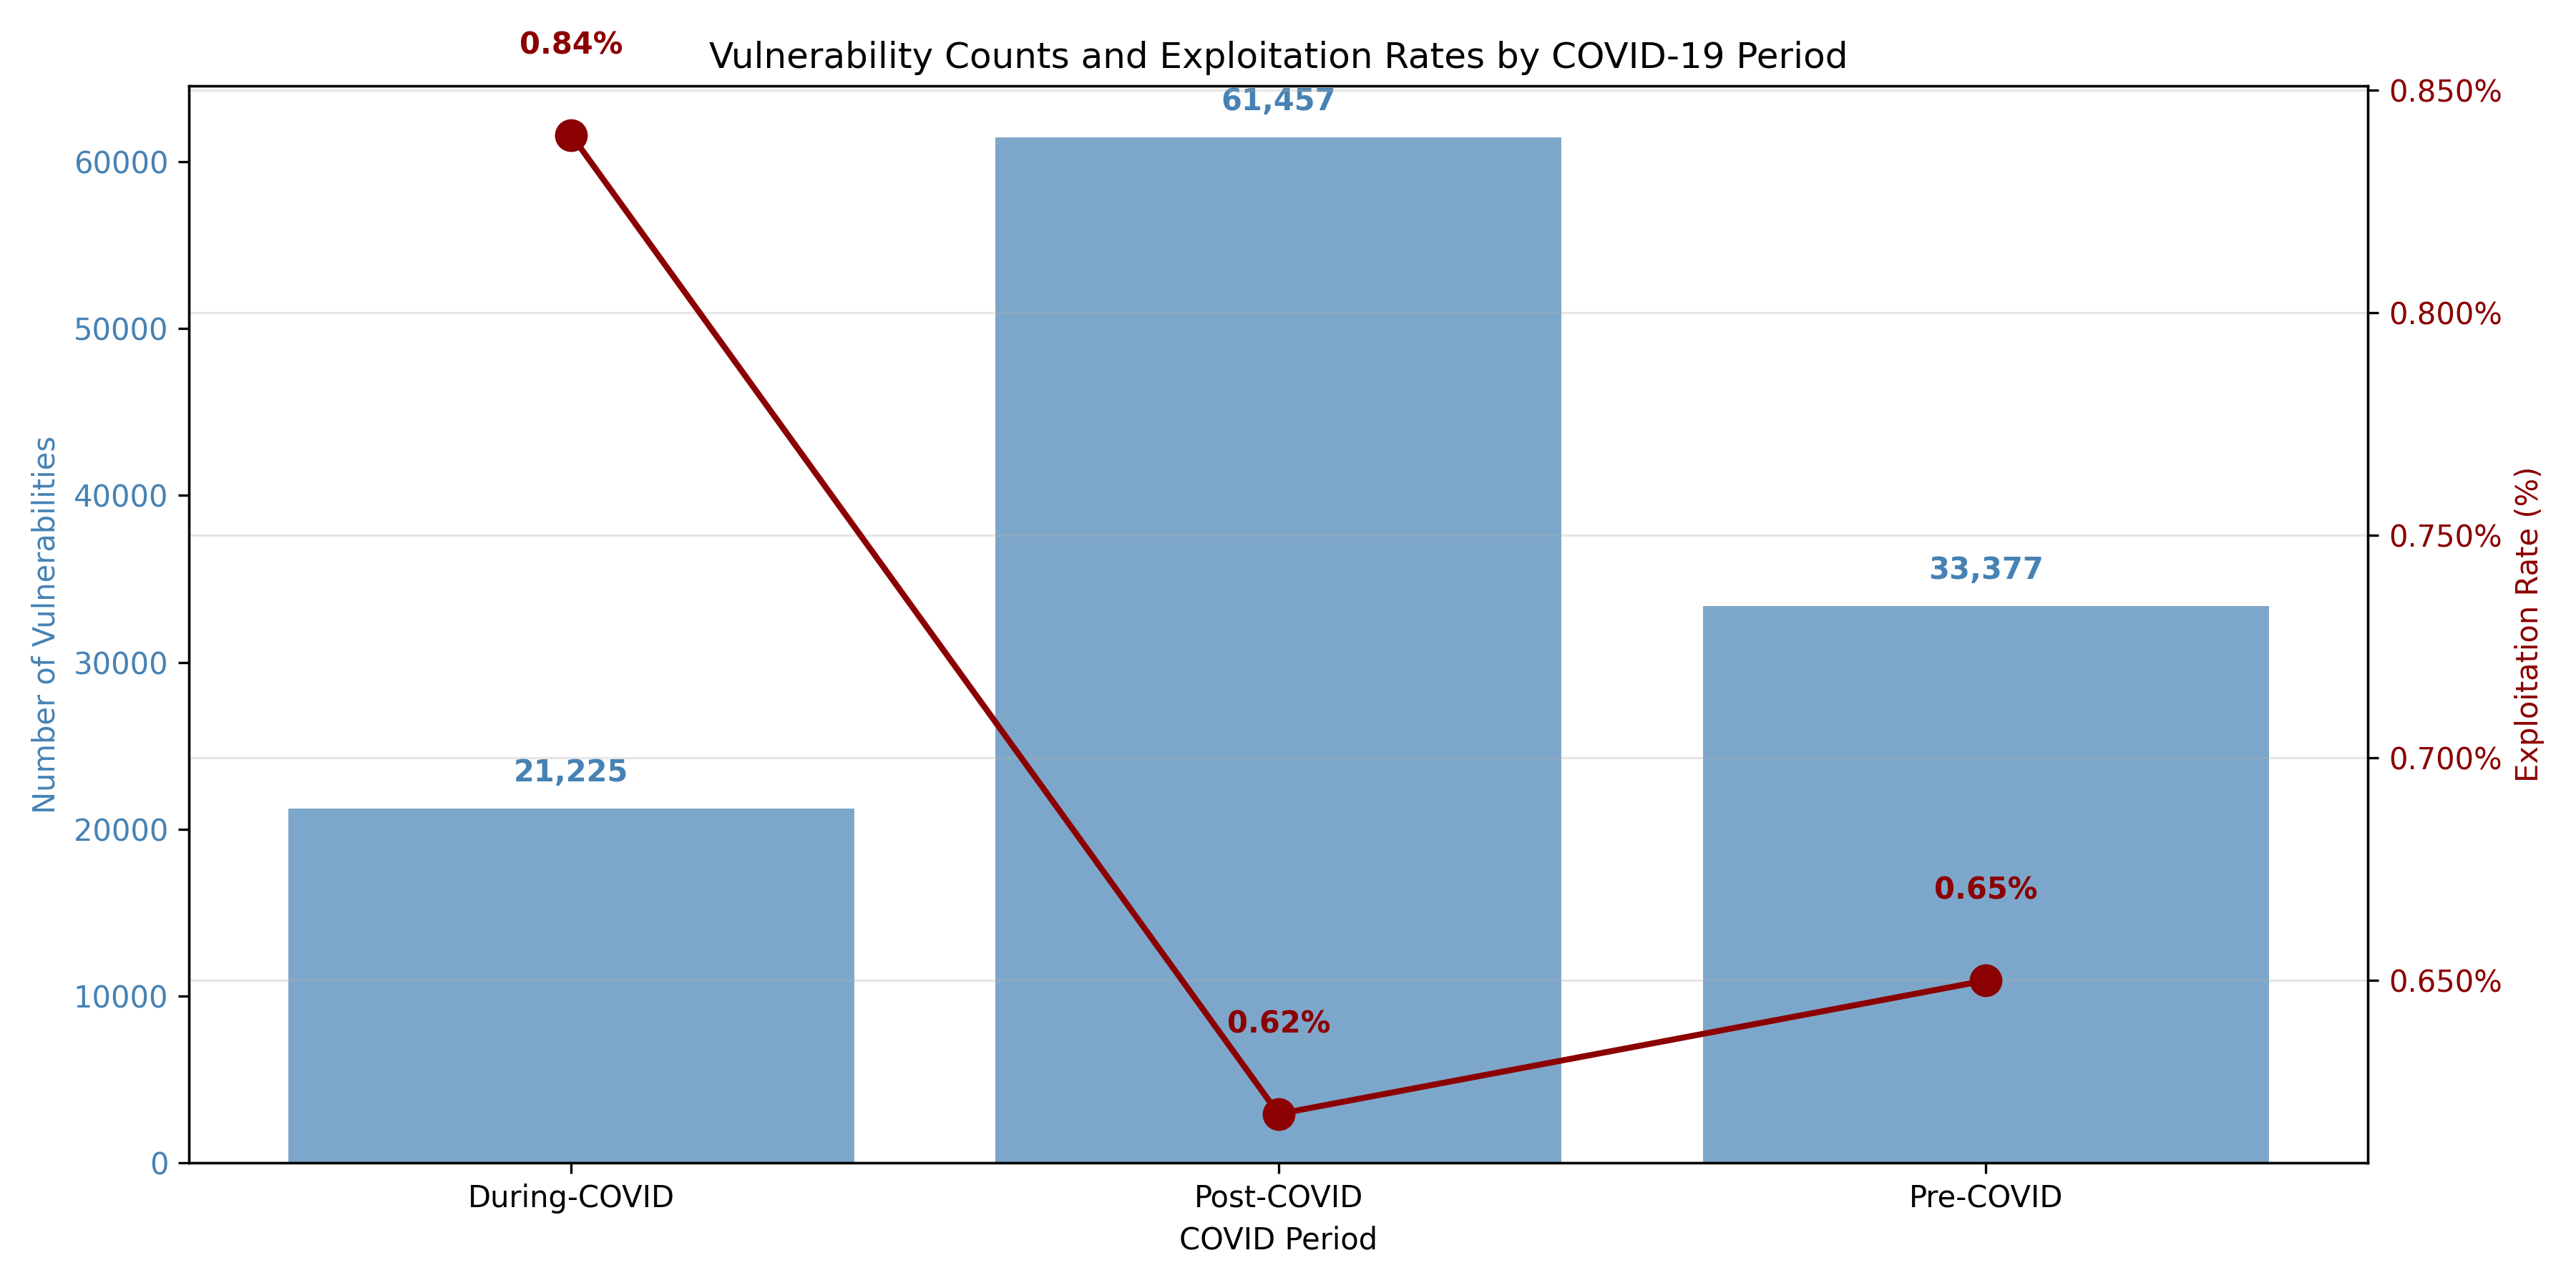
\includegraphics[width=\textwidth]{covid_period_comparison.png}
    \caption{Vulnerability Counts and Exploitation Rates by COVID-19 Period. This dual-axis chart shows both the absolute number of vulnerabilities (blue bars) and their exploitation rates (red line) across pre-COVID, during-COVID, and post-COVID periods.}
    \label{fig:covid_impact}
\end{figure}

\begin{figure}[htbp]
    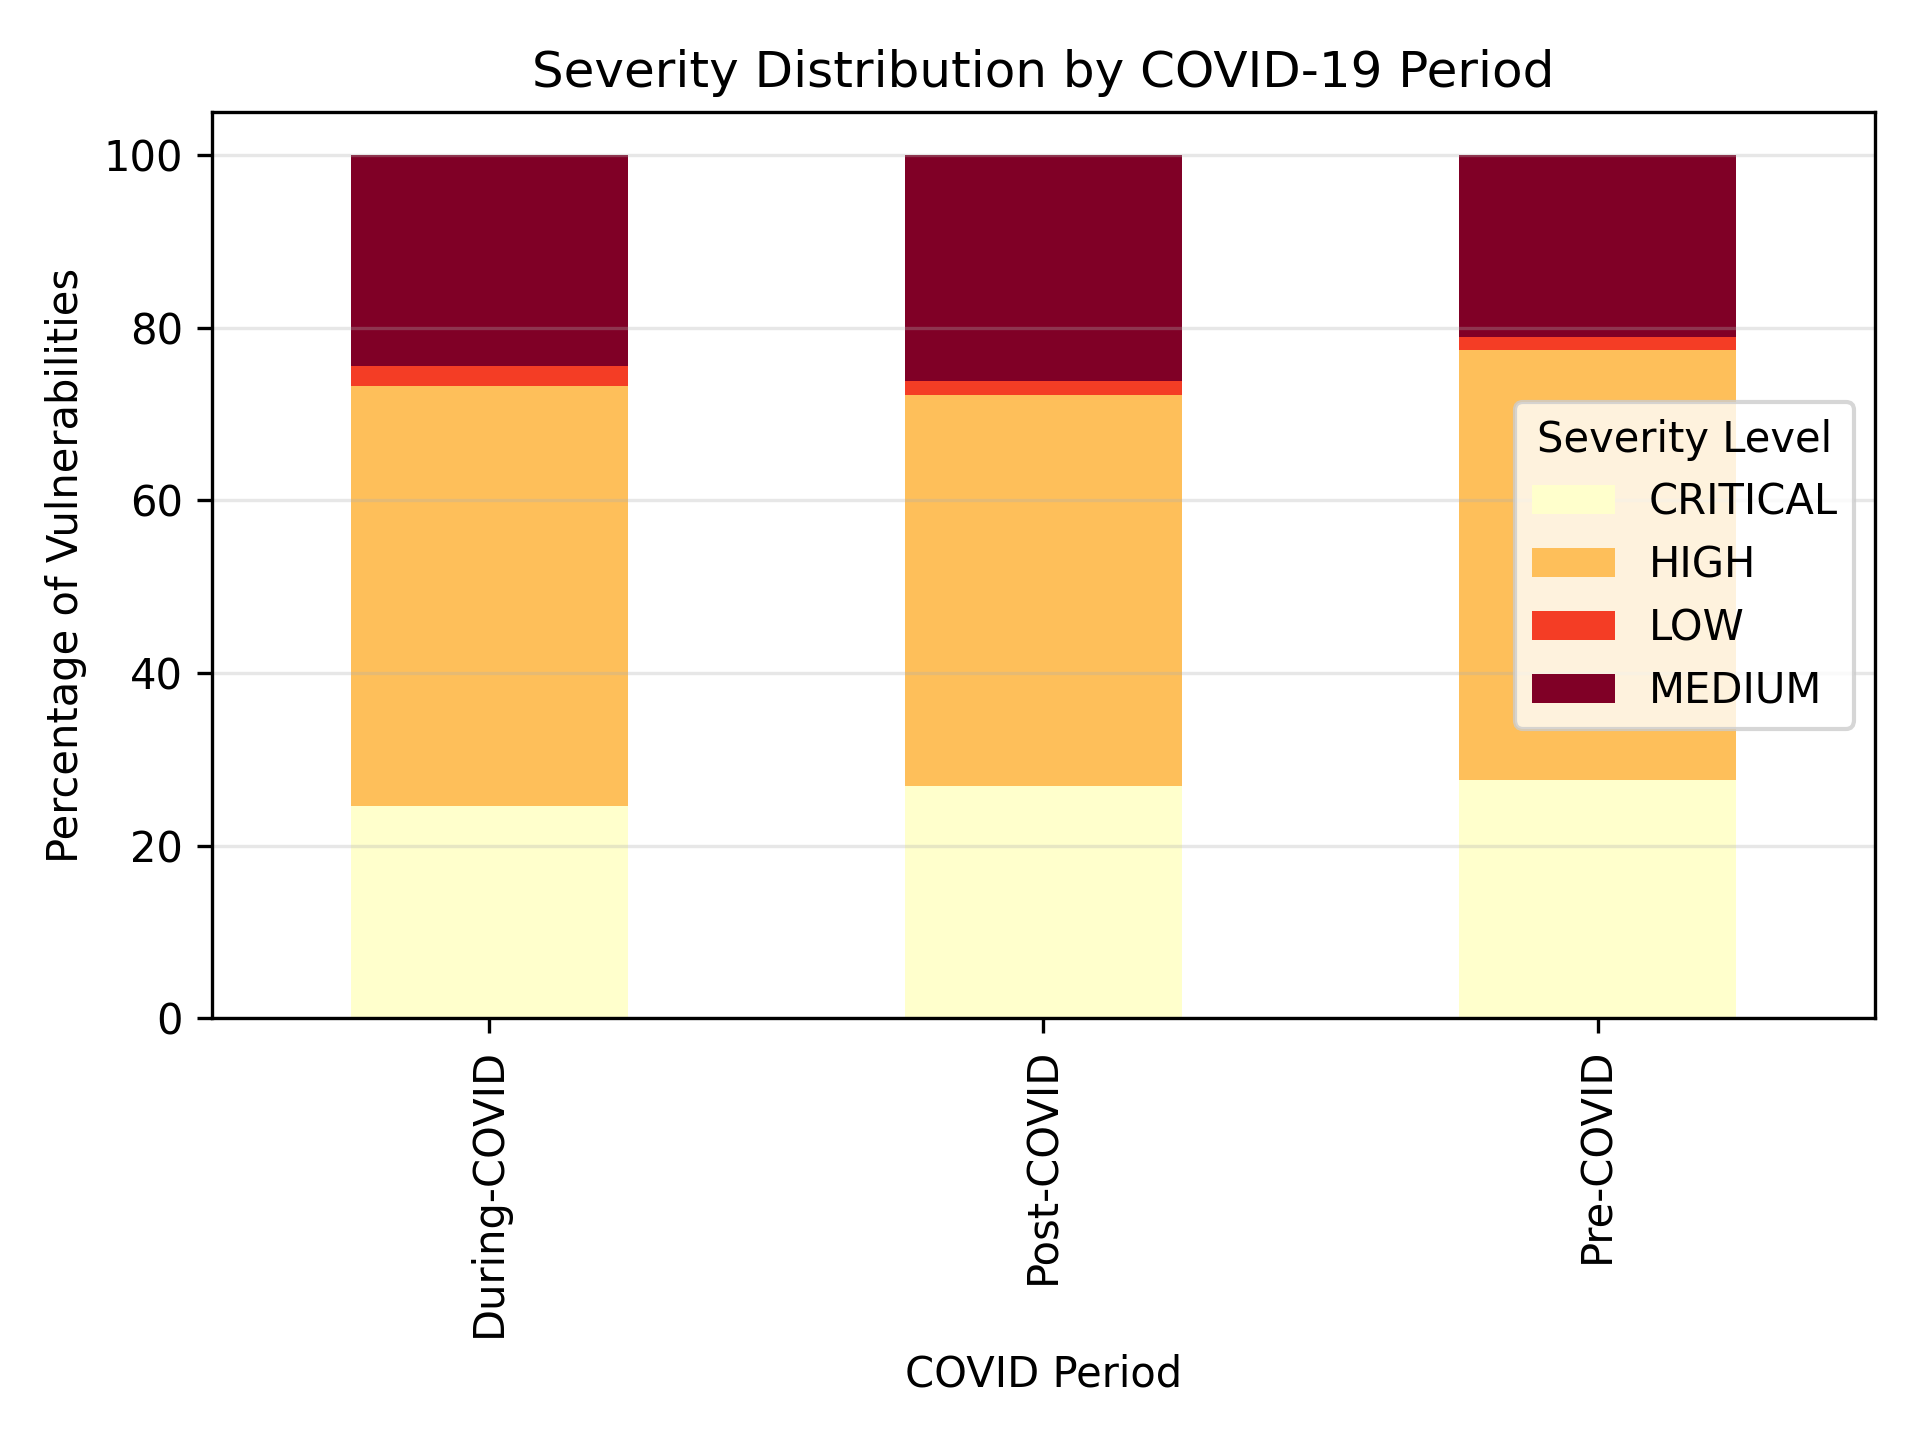
\includegraphics[width=\textwidth]{severity_distribution_covid.png}
    \caption{Severity Distribution by COVID-19 Period. This stacked area chart shows the distribution of vulnerability severity levels during different pandemic phases.}
    \label{fig:severity_distribution}
\end{figure}

\begin{figure}[htbp]
    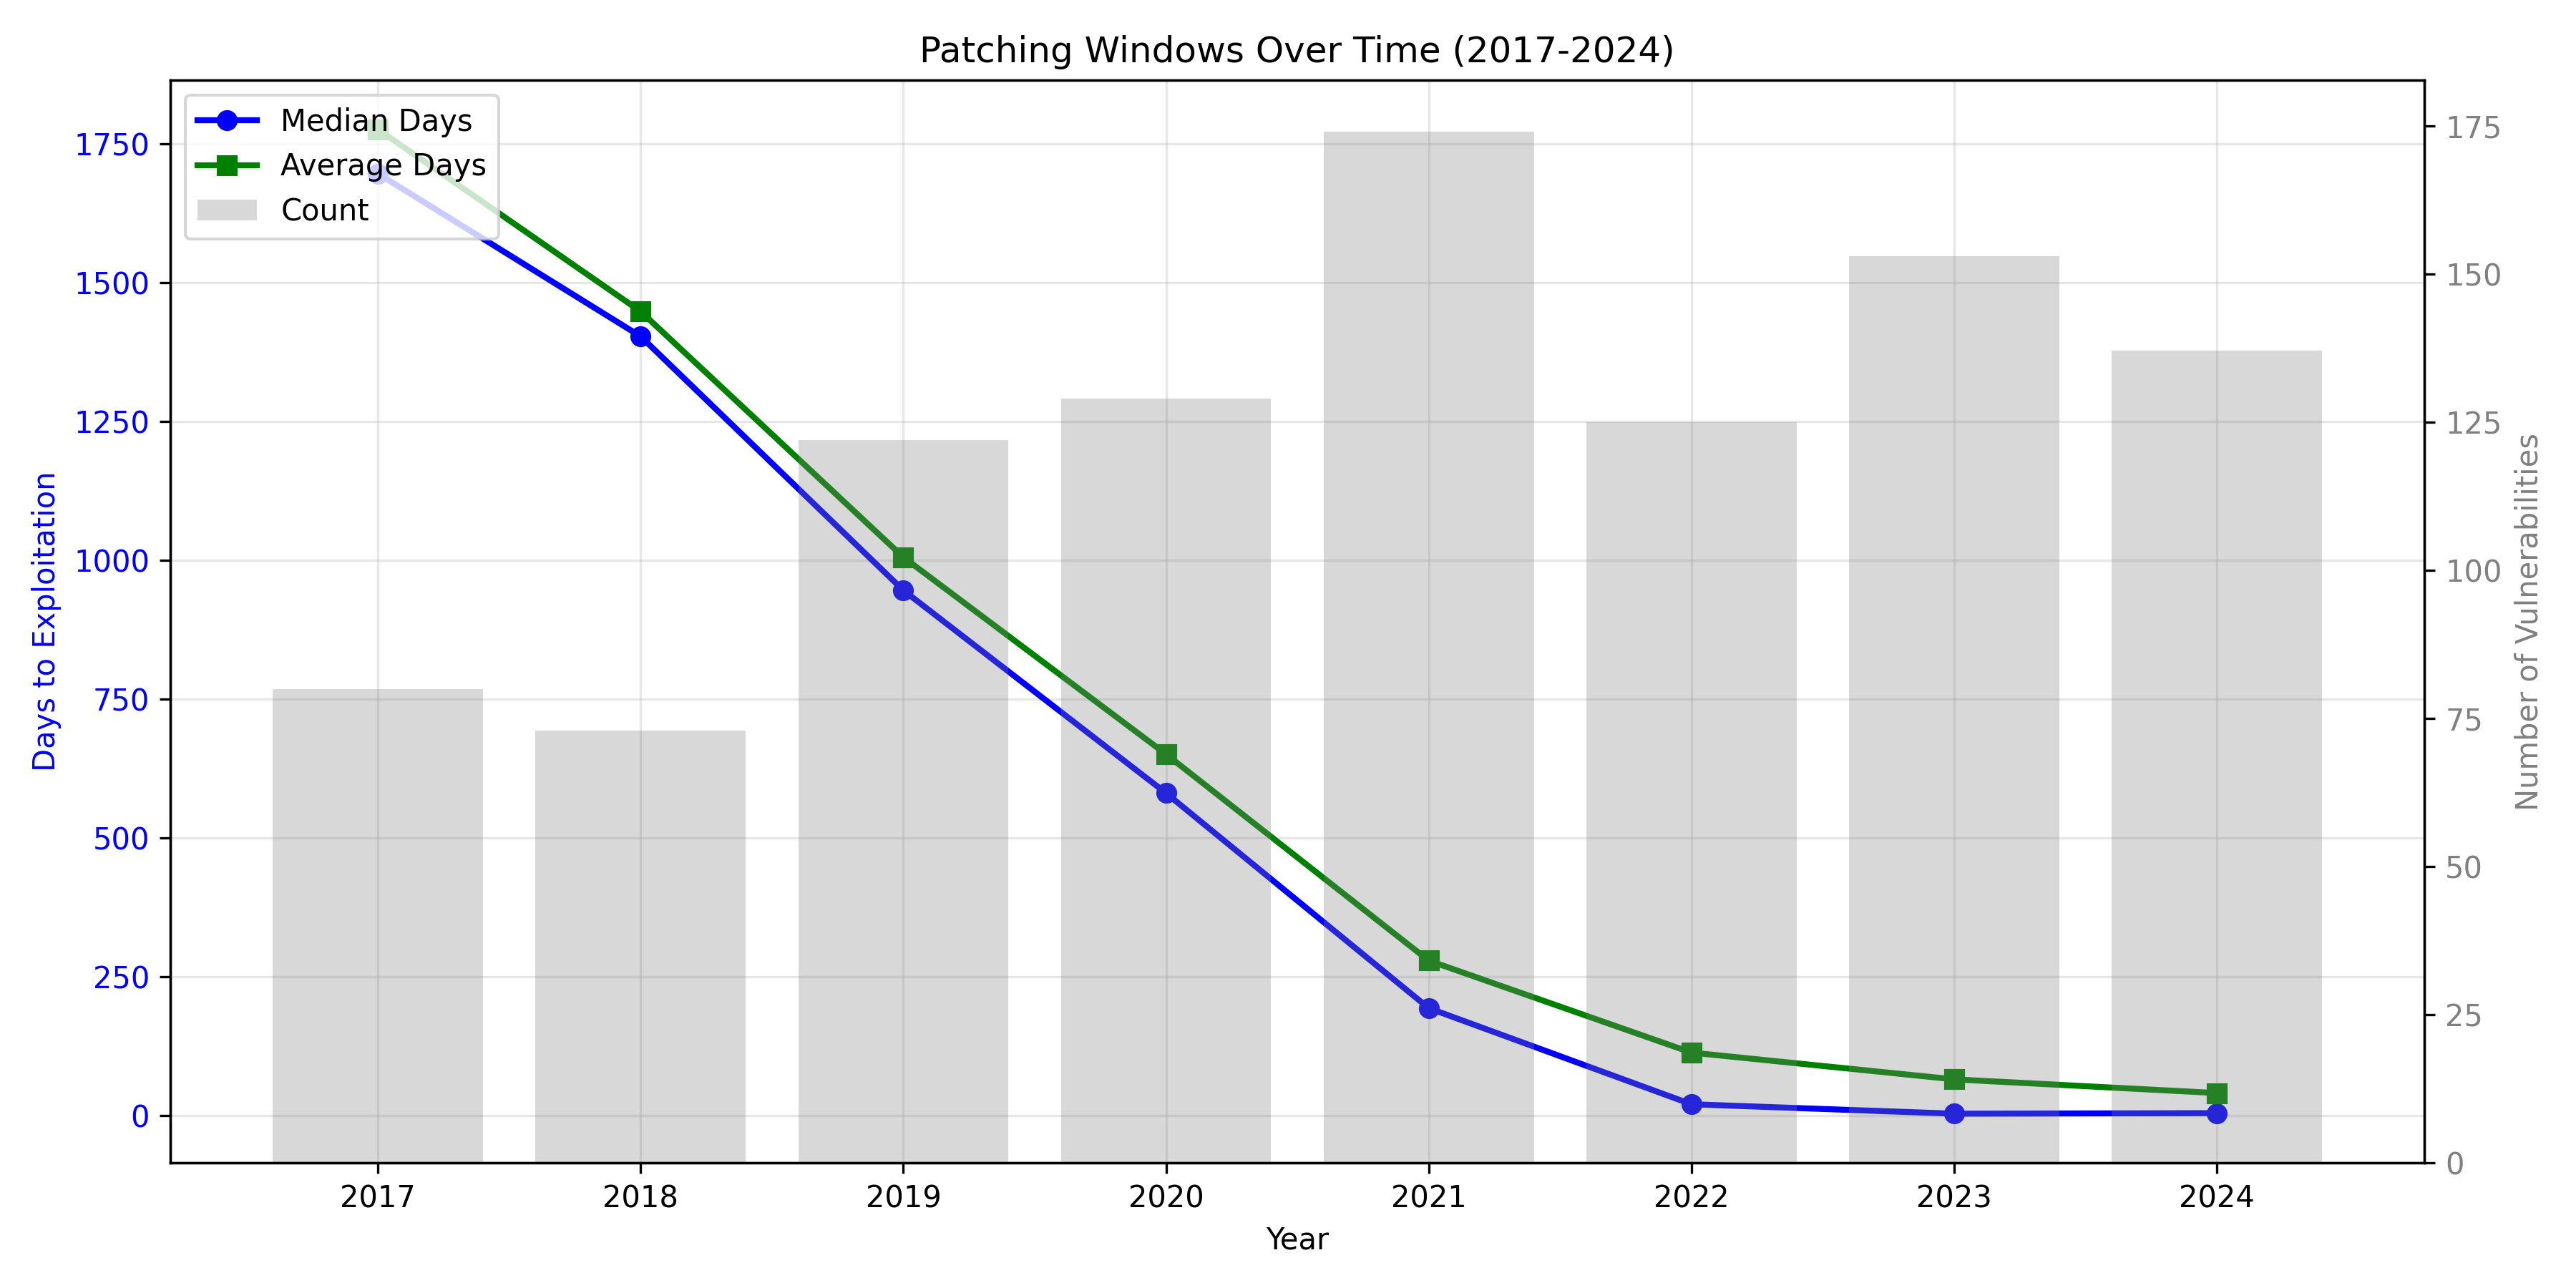
\includegraphics[width=\textwidth]{patching_windows_over_time.png}
    \caption{Patching Windows Over Time (2017-2024). This shows the trend in days to exploitation over time, with vulnerability counts shown in gray bars.}
    \label{fig:patching_windows}
\end{figure}

\begin{figure}[H]
    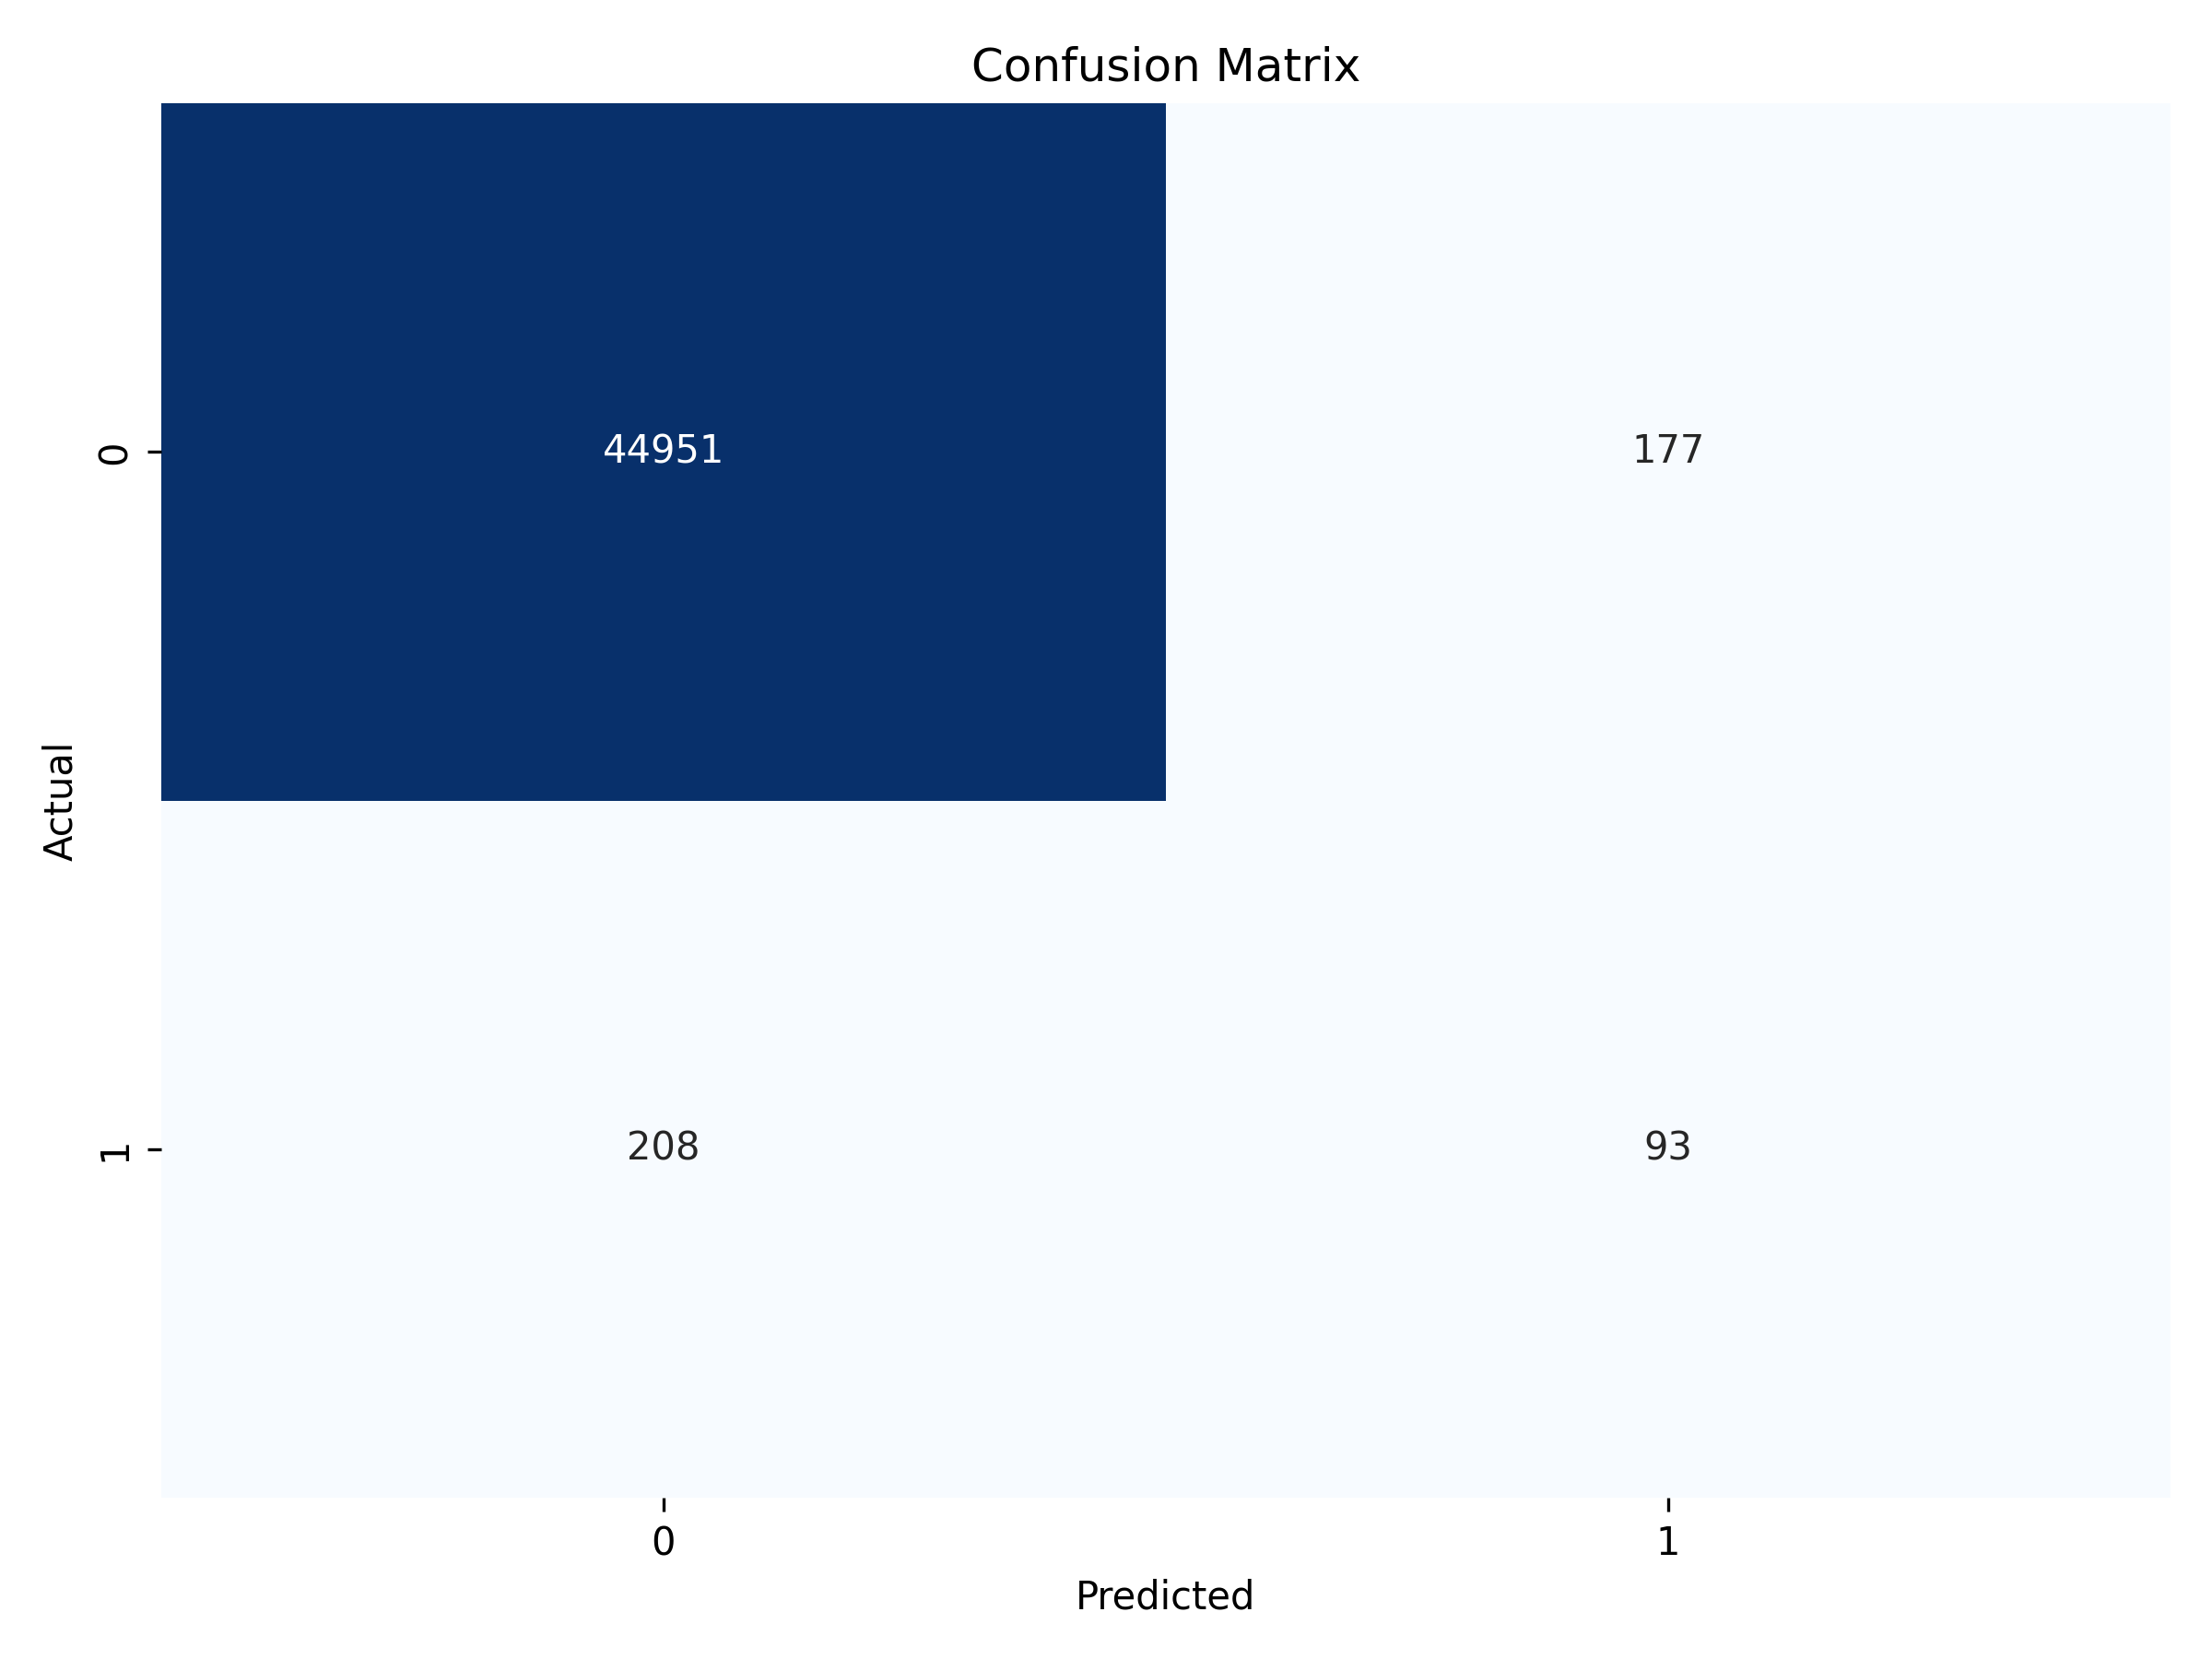
\includegraphics[width=\textwidth]{confusion_matrix.png}
    \caption{Confusion Matrix for Exploitation Prediction. This shows the performance of Random Forest in predicting vulnerability exploitation, with true negatives (44951), false positives (177), false negatives (208), and true positives (93).}
    \label{fig:confusion_matrix}
\end{figure}

\begin{figure}[H]
    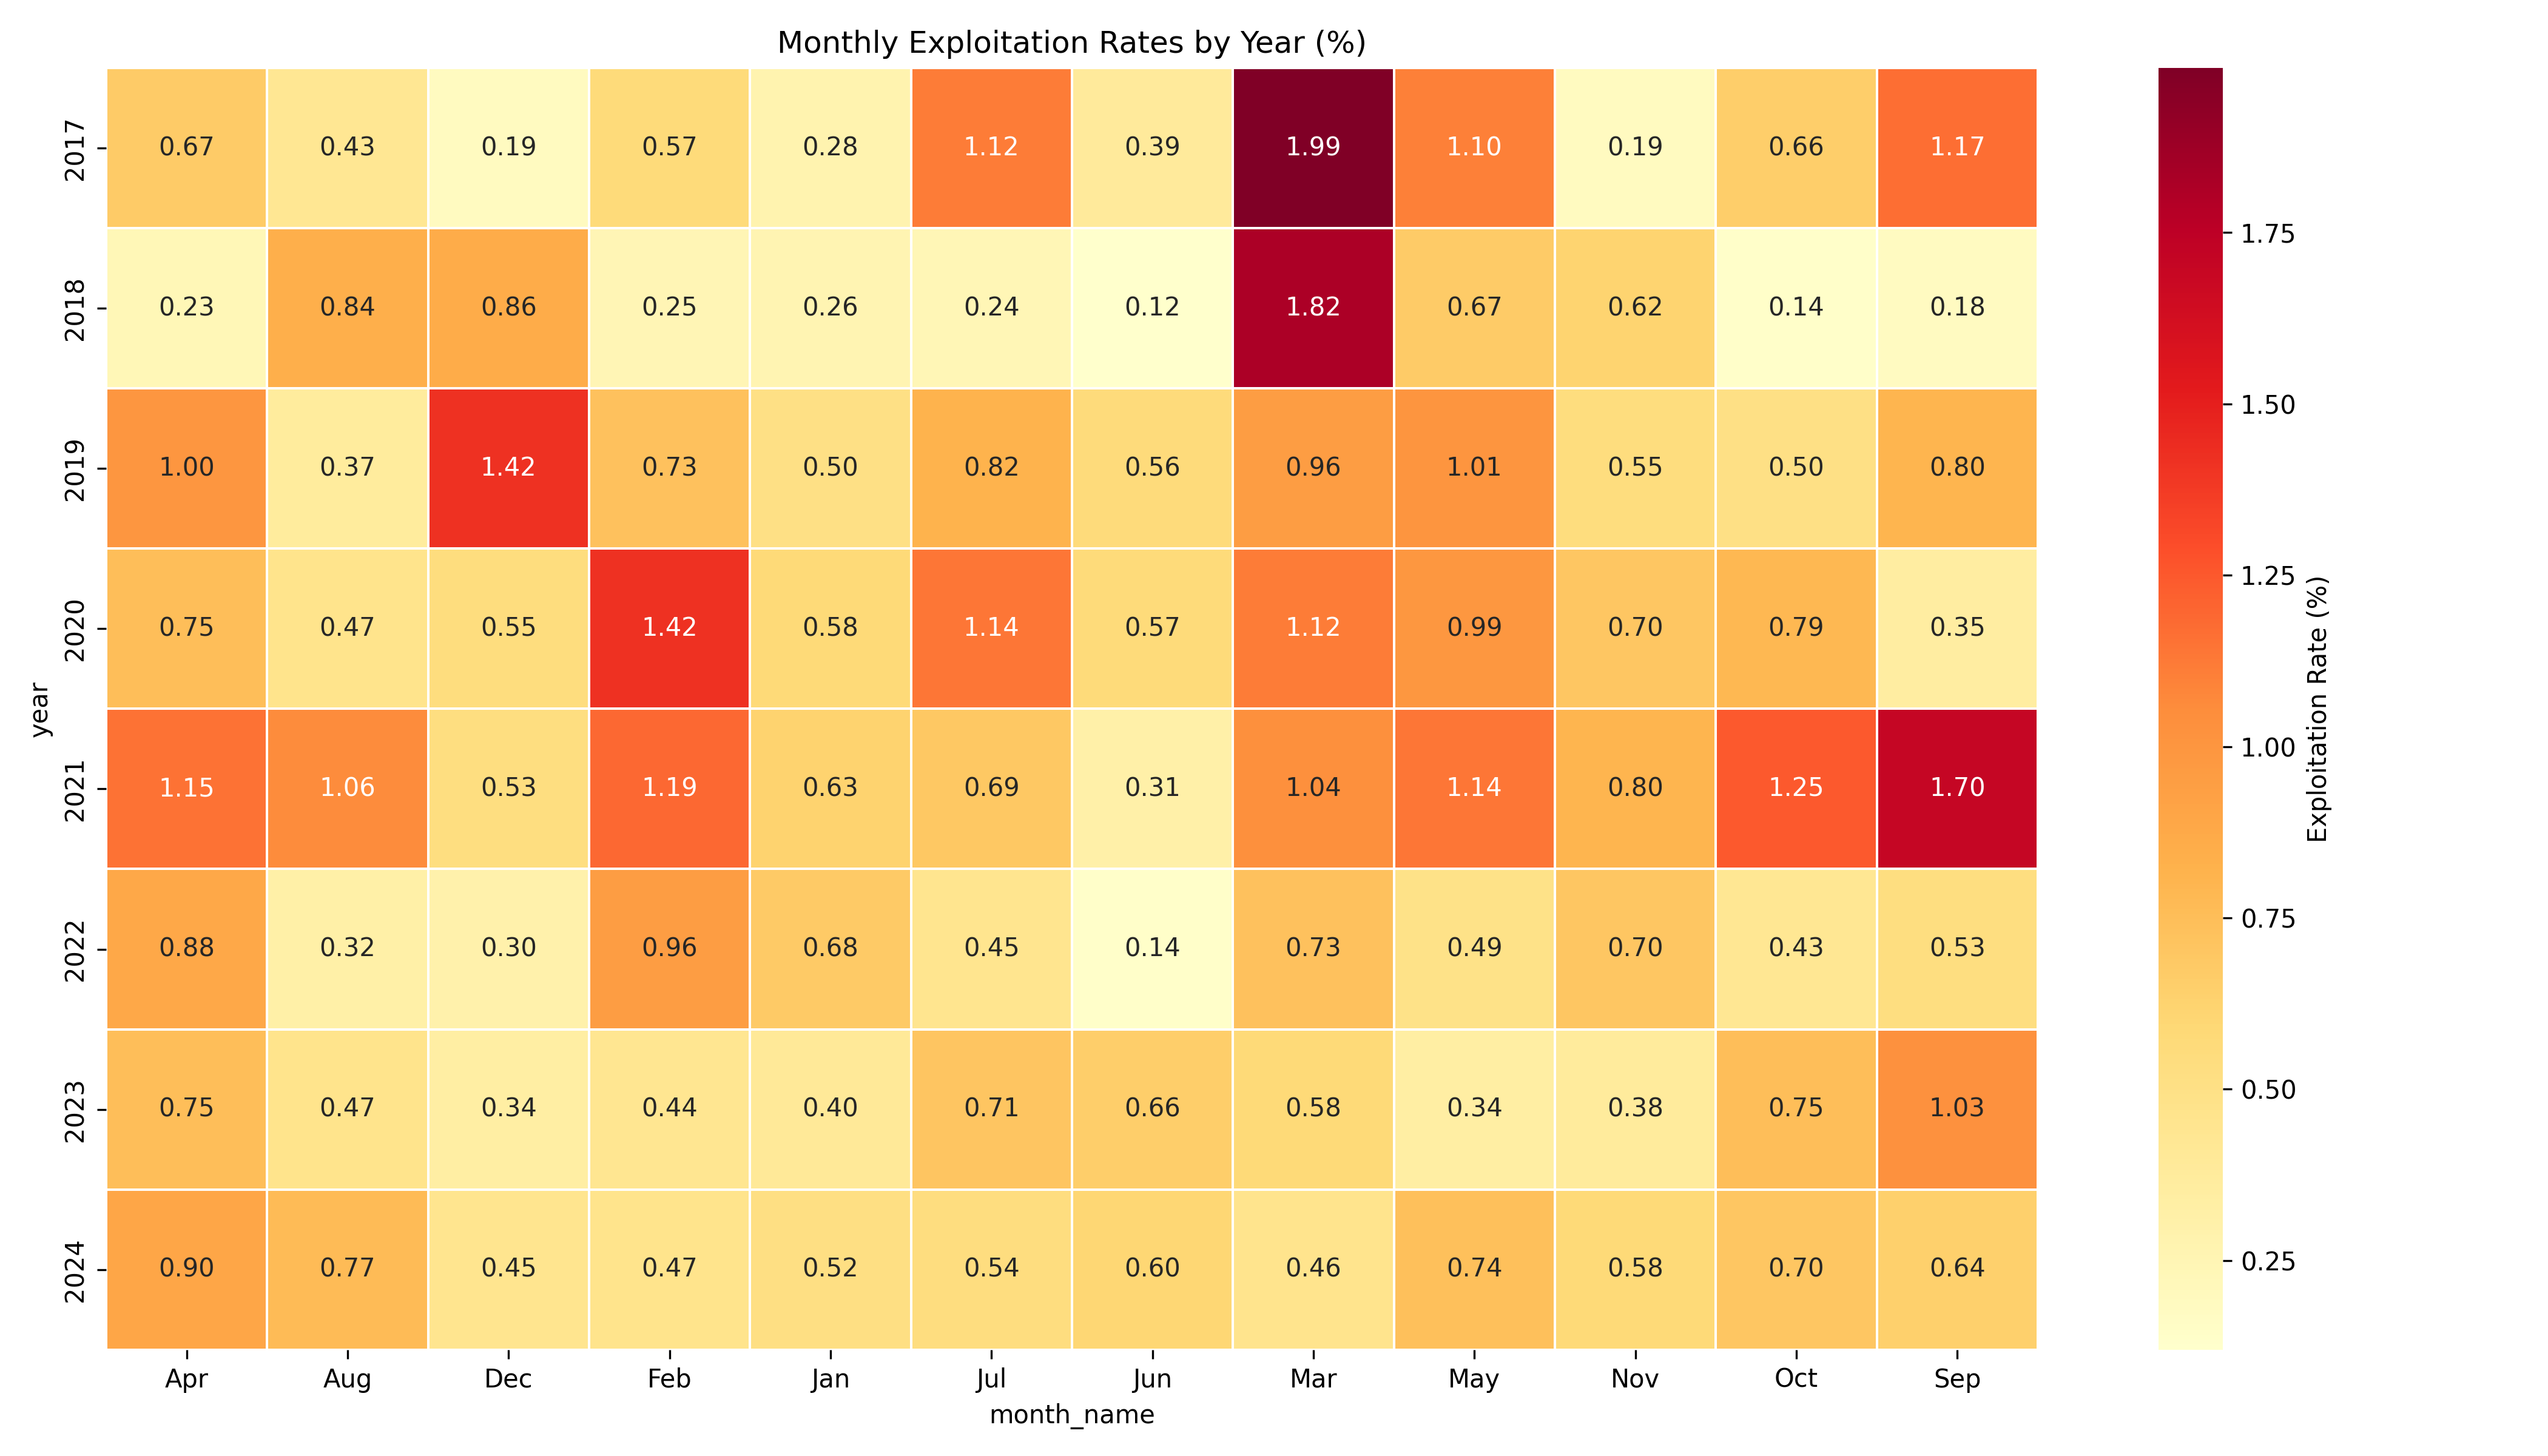
\includegraphics[width=\textwidth]{yearly_monthly_heatmap.png}
    \caption{Monthly Exploitation Rates by Year (\%). This heatmap visualizes exploitation rates for each month across the years. Darker colors indicate higher exploitation rates.}
    \label{fig:monthly_exploitation}
\end{figure}

\begin{figure}[H]
    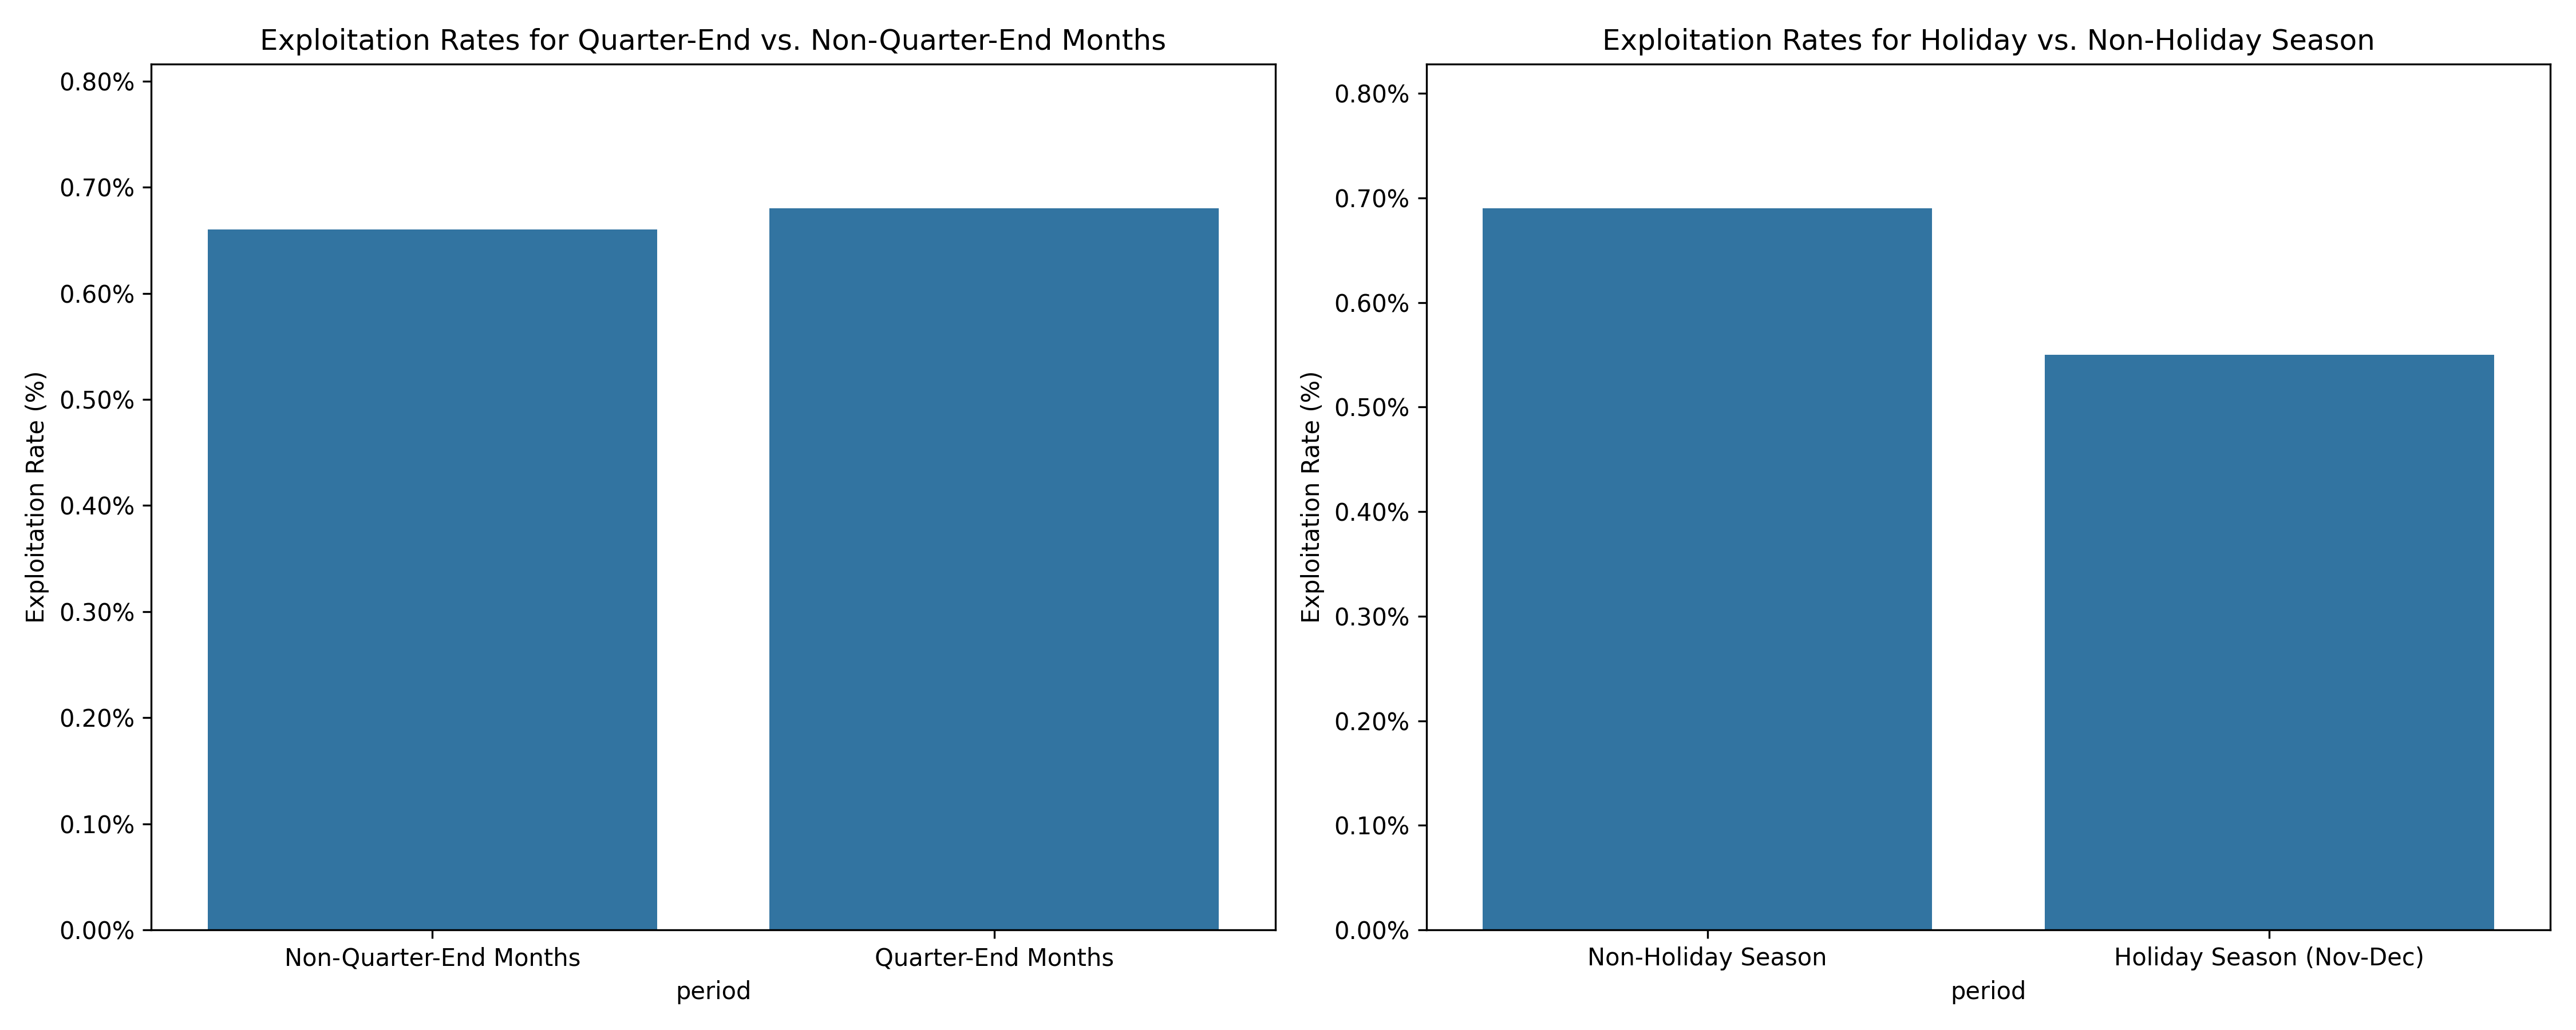
\includegraphics[width=\textwidth]{seasonal_comparisons.png}
    \caption{Exploitation Rates for Quarter-End vs. Non-Quarter-End Months (left) and Holiday vs. Non-Holiday Season (right). These comparative bar charts show the differences in exploitation rates during different business and calendar periods.}
    \label{fig:seasonal_comparison}
\end{figure}

\section{Detailed Results Analysis}
\label{sec:detailed_results}

\subsection{Visualization-Driven Insights}

\subsubsection{COVID-19 Impact Visualization Analysis}
Figure \ref{fig:covid_impact} reveals a striking contrast between vulnerability counts and exploitation rates across pandemic periods. While the post-COVID period shows the highest absolute number of vulnerabilities (61,457), the during-COVID period exhibits the highest exploitation rate (0.84\%), suggesting attackers were more active during the pandemic despite fewer total vulnerabilities.

Figure \ref{fig:severity_distribution} shows that the severity distribution remained relatively consistent across all periods, indicating that the increased exploitation rate during COVID was not due to a shift toward more severe vulnerabilities but rather suggests a change in attacker behavior.

\subsubsection{Temporal Patching Window Analysis}
Figure \ref{fig:patching_windows} displays a clear downward trend in exploitation timing from 2017 to 2024. The median time to exploitation has decreased dramatically from over 1,500 days in 2017 to near-zero in 2023-2024, indicating a fundamental shift in the cybersecurity landscape.

The convergence of mean and median lines in recent years suggests a more uniform exploitation pattern with fewer extreme outliers. This trend has dire implications for organizational security, as the window for remediation continues to shrink.

\subsubsection{Seasonal Pattern Analysis}
The heatmap in Figure \ref{fig:monthly_exploitation} reveals complex temporal patterns in exploitation rates. Certain months (March, August, September) consistently show elevated exploitation rates across multiple years. The highest exploitation rate was observed in March 2017 (1.99\%), while the lowest was in June 2018 (0.12\%).

Figure \ref{fig:seasonal_comparison} shows that contrary to conventional wisdom, the holiday season exhibits lower exploitation rates than the rest of the year. This challenges common security practices and suggests resources might be better allocated to higher-risk periods.

\subsection{Statistical Inferences}
Key statistical inferences include:

\begin{itemize}
    \item The 29.2\% increase in exploitation rates during COVID is statistically significant (p=0.0131).
    
    \item The temporal distribution of patching windows follows a right-skewed distribution with a long tail (median: 260 days, mean: 531.2 days).
    
    \item Monthly exploitation rates show statistically significant variation (p=0.0428) across the calendar year.
    
    \item The model's AUC of 0.80 indicates that the Random Forest classifier is substantially better than random chance at predicting which vulnerabilities will be exploited.
\end{itemize}

\subsection{Data-Driven Conclusions}

\begin{enumerate}
    \item \textbf{Pandemic Impact}: The COVID-19 pandemic created measurable and statistically significant increases in cybersecurity risk, with exploitation rates rising by nearly 30\% during this period, likely due to expanded attack surfaces, reduced security operations efficiency, and attacker opportunism.
    
    \item \textbf{Shrinking Patching Windows}: The dramatic reduction in time-to-exploitation over the past seven years represents a fundamental shift in the threat landscape, requiring organizations to adapt their vulnerability management programs accordingly.
    
    \item \textbf{Predictive Attributes}: The EPSS score \cite{jacobs2019exploit}, CVSS base score \cite{cvss_framework}, and integrity impact are the strongest predictors of exploitation, validating the FIRST organization's methodology.
    
    \item \textbf{Counterintuitive Seasonal Patterns}: The data contradicts common assumptions about high-risk periods, showing that holidays have lower exploitation rates while certain months consistently show higher risk.
\end{enumerate}

\section{Discussion and Implications}
\label{sec:discussion}

\subsection{Practical Security Implications}

\subsubsection{Vulnerability Management Prioritization}
Organizations should consider implementing EPSS score-based triage for vulnerabilities, prioritizing those with high integrity impacts, and developing multi-factor scoring systems that incorporate both severity (CVSS) and exploitation likelihood (EPSS) metrics \cite{seiersen2017practical}. This approach would allow security teams to focus limited resources on the vulnerabilities most likely to be weaponized.

\subsubsection{Patching Timeline Adjustments}
The accelerating pace of exploitation necessitates a reassessment of traditional patching timelines. Critical and high-severity vulnerabilities should be remediated within 7 days of disclosure whenever possible, security teams should implement a tiered patching approach with emergency processes for vulnerabilities with high EPSS scores, and organizations with resource constraints should focus on the 22.6\% of vulnerabilities exploited within 30 days.

\subsubsection{Seasonal Security Planning}
The identification of seasonal patterns enables more strategic allocation of security resources throughout the year. Security operations should increase monitoring and response capabilities during March, reallocate resources from holiday periods to quarter-end periods, and synchronize vulnerability scanning and patching cycles with identified high-risk periods.

\subsection{Theoretical Contributions}
This research makes several theoretical contributions to the field of cybersecurity:

\begin{itemize}
    \item \textbf{Exploitation Lifecycle Model}: The findings support a refined model of vulnerability exploitation that includes pre-disclosure, critical window, mainstream, and long-tail phases.
    
    \item \textbf{Attacker Behavior Theory}: The seasonal patterns and COVID-19 impact analysis provide evidence that attacker behavior is influenced by both opportunity and capacity, rather than simply following fixed seasonal cycles.
    
    \item \textbf{Vulnerability Attractiveness Framework}: The predictive model identifies specific characteristics that make vulnerabilities attractive to attackers.
\end{itemize}

\subsection{Methodological Innovations}
The research methodology presented several innovations:

\begin{itemize}
    \item The integration of multiple data sources provides a more comprehensive view of the vulnerability lifecycle than any single source could offer.
    
    \item The application of machine learning to highly imbalanced cybersecurity datasets demonstrates effective approaches to addressing the rare event prediction problem.
    
    \item The temporal analysis approach, combining absolute counts with relative rates, offers a more nuanced understanding of risk patterns.
\end{itemize}

\subsection{Unexpected Findings}
Several findings contradicted conventional wisdom in cybersecurity:

\begin{itemize}
    \item High-complexity vulnerabilities are more frequently exploited than low-complexity ones, challenging the assumption that attackers consistently prioritize ease of exploitation.
    
    \item The reduced exploitation activity during holiday periods contradicts common security practices.
    
    \item The dramatic acceleration in exploitation timing suggests that industry standards for "reasonable" patching windows may be increasingly outdated.
\end{itemize}

\section{Conclusion and Future Work}
\label{sec:conclusion}

\subsection{Summary of Key Findings}
This research has provided empirical evidence on four key aspects of vulnerability exploitation:

\begin{enumerate}
    \item \textbf{Seasonal Patterns}: Exploitation rates vary significantly by month, with March showing the highest risk (0.95\%) and June the lowest (0.42\%).
    
    \item \textbf{Critical Patching Windows}: The median time to exploitation is 260 days, but 17.1\% of exploitations occur within 7 days of disclosure.
    
    \item \textbf{Predictive Attributes}: The EPSS score, CVSS base score, HIGH integrity impact, and the presence of public exploits are the strongest predictors of exploitation.
    
    \item \textbf{COVID-19 Impact}: The pandemic period showed a statistically significant 29.2\% increase in exploitation rates compared to the pre-pandemic baseline.
\end{enumerate}

\subsection{Limitations}
Despite its contributions, this research has several limitations:

\begin{itemize}
    \item Reliance on publicly reported exploitation data, which likely underrepresents the true scope of exploitation activity.
    \item Arbitrary time boundaries for COVID-19 period analysis that may not perfectly align with actual pandemic effects.
    \item Modest performance metrics on the positive class (precision: 0.34, recall: 0.31), indicating room for improvement in exploitation prediction.
    \item Dataset limited to vulnerabilities from 2017-2024, which may not fully capture longer-term trends.
\end{itemize}

\subsection{Future Research Directions}
Several promising avenues for future research emerge from this work:

\begin{itemize}
    \item \textbf{Advanced Predictive Models}: Developing ensemble models or deep learning approaches to improve prediction performance for rare exploitation events.
    
    \item \textbf{Finer-Grained Temporal Analysis}: Examining weekly or daily exploitation patterns to identify micro-trends.
    
    \item \textbf{Organizational Factors}: Investigating how organizational characteristics influence vulnerability exploitation rates and patterns.
    
    \item \textbf{Attacker Economics}: Exploring the economic drivers behind exploitation patterns.
    
    \item \textbf{Exploitation Cascades}: Analyzing how exploitation of one vulnerability affects the likelihood of exploitation for related vulnerabilities.
\end{itemize}

\subsection{Concluding Remarks}
This research demonstrates that vulnerability exploitation follows discernible patterns that can be identified, quantified, and predicted through data-driven analysis. The findings challenge several common assumptions in cybersecurity practice and offer concrete guidance for improving vulnerability management strategies.

The dramatic acceleration in exploitation timing, the clear impact of global events like the COVID-19 pandemic, and the identification of specific vulnerability attributes that predict exploitation all point to a security landscape that is continuously evolving but can be better understood through empirical analysis.

By incorporating these insights into security operations, organizations can move from reactive to proactive security postures, allocating limited resources more effectively to address the vulnerabilities that pose the greatest actual risk.

\section{Supplemental Materials from GitHub}
\label{sec:supplemental_materials}

The following links provide additional context and source code for the predictive attributes analysis:

\begin{itemize}
    \item \textbf{Project Repository:} \url{https://github.com/gjrich/ms-capstone/}
    
    \item \textbf{Script generating the results:} \\\url{https://github.com/gjrich/ms-capstone/blob/master/problems/predictive_attributes.py}

    \item \textbf{Basic results (log file):} \\\url{https://github.com/gjrich/ms-capstone/blob/master/problems/predictive_attributes.txt}

    \item \textbf{Images detailing the analysis results:} \\\url{https://github.com/gjrich/ms-capstone/tree/master/problems/analysis_results/predictive}
\end{itemize}

These materials complement the discussion in Section~\ref{sec:implementation_evaluation}, providing both the raw output and visualizations of the model's performance.

\bibliographystyle{splncs04}
\bibliography{mybibliography}

\end{document}